\documentclass[main]{subfiles}
\begin{document}

\centering
\logo \\[3em]
\textbf{\LARGE \universityname} \\[1em]
\textbf{\Large \facultyname} \\[1em]
\textbf{\large \departmentname} \\[3em]
\textbf{\Huge \projecttitle} \\[2em]
\textbf{\Large By} \\[1em]
\begin{tabular}[pos]{c} 
    \textbf{\uppercase{hashem vaseghi}}      \\[0.5em] 
    \textbf{\uppercase{Parfait Zaina Ngoi}}  \\[0.5em]
    \textbf{\uppercase{Felly Ngoy}}          \\[0.5em]
    \textbf{\uppercase{Jude Kabemba}}        \\[0.5em]
    \textbf{\uppercase{Boima Fahnbulleh}}   \\[0.5em]
    \textbf{\uppercase{Gregory Mwema}}     \\[0.5em]
    \textbf{\uppercase{Olutoye Opeyemi}}   \\[0.5em]
\end{tabular}
\vfill
\textbf{\reportdate} \\[1em]
\textbf{\reportplace} \\[1em]
%this is table of content
\pagenumbering{gobble}

\newpage

\centering
\logo \\[3em]
\textbf{\LARGE \universityname} \\[1em]
\textbf{\Large \facultyname} \\[1em]
\textbf{\large \departmentname} \\[3em]
\textbf{\Huge \projecttitle} \\[2em]
\textbf{\Large By} \\[1em]
\begin{tabular}[pos]{c} 
    \textbf{\uppercase{hashem vaseghi}}      \\[0.5em]
    \textbf{\uppercase{Parfait Zaina Ngoi}}  \\ [0.5em]
    \textbf{\uppercase{Felly Ngoy}}          \\ [0.5em] 
    \textbf{\uppercase{Jude Kabemba}}        \\ [0.5em]
    \textbf{\uppercase{Boima Fahnbulleh}}   \\[0.5em]
    \textbf{\uppercase{Gregory Mwema}}     \\[0.5em]
    \textbf{\uppercase{Olutoye Opeyemi}}   \\[0.5em]
\end{tabular}
\vfill
\textbf{\reportdate} \\[1em]
\textbf{\reportplace} \\[1em]
%this is table of content

\newpage

\centering
\textbf{\LARGE \projecttitle} \\[1em]

\textbf{\Large By} \\[3em]
\begin{tabular}[pos]{c c c} \hline
    Hashem Vaseghi     & 22004087 & Electrical and Electronic Engineering \\ 
    Parfait Zaina Ngoi & 22015208 & Electrical and Electronic Engineering \\
    Felly Ngoy         &22013357& Computer Engineering \\
    Jude Kabemba       &22013160& Computer Engineering \\
    Boima Fahnbulleh  & 22013081 & Mechatronics Engineering \\
    Gregory Mwema    & 22012501& Mechatronics Engineering \\
    Olutoye Opeyemi  &22013786& Mechanical Engineering \\
\end{tabular}\\[10em]
{\raggedright
\textbf{DATE OF APPROVAL: ................}\\[2em]
APPROVED BY: \\[4em]
\textbf{\supe} \\[2em]
{\raggedleft
\textbf{ \rule{5cm}{0.4pt} }\\[7em]}
\textbf{\supm} \\[2em]
{\raggedleft
\textbf{ \rule{5cm}{0.4pt} }\\[2em]}
\vfill
%this is table of content
}
\newpage

\pagenumbering{Roman}


\chapter*{\hfill ACKNOWLEDGEMENTS \hfill}

\justifying % Justify text
We extend our heartfelt appreciation to everyone who contributed to the success of this project. First and foremost, we express our deepest gratitude to \textbf{Asst. Prof. Dr. ZİYA DEREBOYLU} and \textbf{Asst. Prof. Dr. ALİ SHEFIK} for their invaluable guidance, continuous support, and encouragement throughout the project. Their expertise and insights were instrumental in overcoming challenges and ensuring the project's progress.

We are also grateful to \textbf{Cyprus International University} for providing us with the resources and platform to pursue this project. Special thanks to the faculty members of the \textbf{Faculty of Engineering} for their technical advice and mentorship, which greatly enriched our learning experience.

Our sincere thanks go to our entire team for their dedication and collaboration. Each member brought unique skills and perspectives, contributing to the successful integration of mechanical, electronic, and software systems. This project would not have been possible without their united commitment and hard work.

We also extend our gratitude to our families and friends for their unwavering support, encouragement, and motivation during the challenging phases of the project.

Finally, we would like to thank the organizers of the Teknofest Aerospace and Technology Festival for providing us with the opportunity to showcase our work and compete in the Digital Technologies in Industry competition.

This project is a testament to the collective effort and support of everyone involved. Thank you all for being part of this journey.
\newpage
\centering
\chapter*{\hfil ABSTRACT \hfil}
\justifying
The research introduces CIU\_Fox as an autonomous guided vehicle (AGV) that develops capabilities to transform factory and warehouse internal transportation operations. The designed AGV features autonomous navigation with a safe lifting capability using obstacle detection and collision avoidance systems for moving loads up to 200 kg.
This system combines LIDAR with time-of-flight (ToF) sensors and barcode scanners to create a precise automated navigation system which monitors operations and handles loading duties.
The mechanical structure incorporates an aluminum alloy frame together with a scissor-compartment mechanism and NEMA 23 stepper-motor powered differential steering.
A Raspberry Pi 4 manages the system through ESP32 modules that run software programs built in Python and C++ within the ROS framework.
The robot development followed four sequential stages that led to its physical assembly. Resources limitations required the project team to conduct final stage testing through the Gazebo simulation pipeline instead of building physical components. Coding for path planning alongside obstacle avoidance and load management functions while achieving complete integration of mechanical electronic software system components stands as major accomplishments. The commercial application scope of the AGV remains promising in multiple industrial sectors including manufacturing storage facilities and logistics operations because it shows potential to optimize operational efficiency while decreasing expenses and protecting worker safety.  
This work illustrates why interdisciplinary teams need to bring innovative solutions to modern industrial design using state-of-the-art technology applications. Research efforts will focus simultaneously on two fronts which include enhancing the AGV's operational excellence while evaluating opportunities to connect it with broader industrial system networks.

\newpage
\centering
\chapter*{\hfil Özet \hfil}
\justifying
Araştırma, fabrika ve depo içi taşıma operasyonlarını dönüştürme yetenekleri geliştiren özerk bir yönlendirmeli araç (AGV) olarak CIU\_Fox'u tanıtmaktadır. 
Tasarlanan AGV, 200 kg'a kadar yük taşıyabilmek için engel algılama ve çarpışma önleme sistemleriyle donatılmış güvenli kaldırma kabiliyetine sahip otonom navigasyon özellikleri sunar.

Bu sistem, operasyonları izleyen ve yükleme görevlerini gerçekleştiren hassas bir otomatik navigasyon sistemi oluşturmak için LIDAR, zaman-uçuşu (ToF) sensörleri ve barkod tarayıcıları birleştirir. 
Mekanik yapı, alaşımlı alüminyum çerçeve, makaslı kompartman mekanizması ve NEMA 23 step motorla çalışan diferansiyel yönlendirme sistemi içerir.

Sistem, ROS çerçevesinde Python ve C++ ile geliştirilen yazılım programlarını çalıştıran ESP32 modülleri aracılığıyla bir Raspberry Pi 4 tarafından yönetilir. 
Robot geliştirme süreci, fiziksel montaja kadar uzanan dört aşamalı bir sırayla tamamlanmıştır. 
Kaynak kısıtlamaları nedeniyle fiziksel bileşenler yerine Gazebo simülasyon ortamında son aşama testleri \\ gerçekleştirilmiştir. 
Yol planlama, engel önleme ve yük yönetimi fonksiyonlarının kodlanması ile mekanik-elektronik-yazılım bileşenlerinin tam entegrasyonu projenin temel başarıları arasındadır.

AGV'nin ticari uygulama kapsamı, üretim tesisleri, depolama alanları ve lojistik operasyonlar gibi çeşitli endüstriyel sektörlerde operasyonel verimliliği artırma, maliyetleri düşürme ve işçi güvenliğini koruma potansiyeli nedeniyle umut vaat etmektedir. 
Bu çalışma,\\ disiplinlerarası ekiplerin en son teknoloji uygulamalarını kullanarak endüstriyel tasarıma yenilikçi çözümler getirmesi gerektiğini vurgulamaktadır. Araştırma çabaları, AGV'nin operasyonel mükemmelliğini artırmanın yanı sıra endüstriyel sistem ağlarına bağlanma fırsatlarını değerlendirmek üzere iki paralı hedefe odaklanacaktır.
\justifying

\newpage
\centering
\tableofcontents
\newpage

\listoffigures
\newpage

\listoftables
\newpage

\listofcodeblocks
\newpage
%nex page is the report
\pagenumbering{arabic}
\chapter{\hfil INTRODUCTION \hfil}
\justifying
\subfile{sublatex/hashem/Teknofest}
\newpage
\centering
\chapter{\hfil LITERATURE SURVEY \hfil}
\justifying
Today’s industries activity have merged
with the robotic and automation world and
day by day having the precise and betterquality
product make the sense of using
new technology. Between all types of
robot, the AGV (automated guided
vehicle) robot has the special place
between others and improvement in
technology helps this design to grow and
become more helpful in various
applications. The AGV robot is a
programmable mobile robot integrated
sensor device that can automatically
perceive and move along the planned
path\cite{das2016design} This system consists of various
parts like guidance facilities, central
control system, charge system and
communication system\cite{moshayedi2019agv}. 

The initial used and Invention AGV is not clear exactly and
was mentioned in different articles and
reference for many times but the earliest
time of using this system in industries is
mentioned in 1950s \cite{reveliotis2000conflict}
(\cref{oldAgv}) and even
mentioned in some reference that the first
AGV in the world was introduced in UK in
1953 for transporting which was modified
from a towing tractor and can be guided by
an overhead wire \cite{moshayedi2019agv}.

\begin{figure}[H]
    \centering
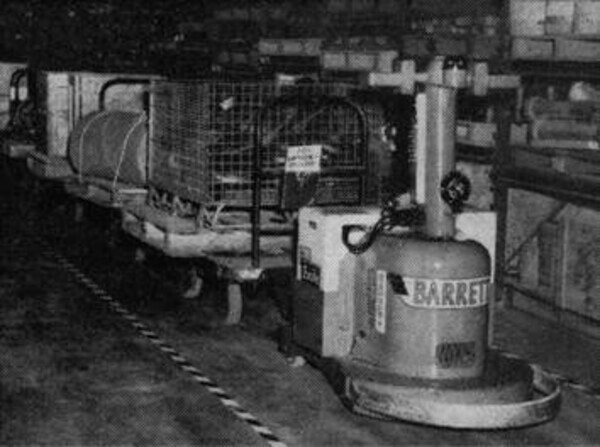
\includegraphics[width=0.5\textwidth]{doc/oldestAGV.jpg}
\caption{one of the Old AGV picture}
\label{oldAgv} % Unique label for referencing
\end{figure}

AGVs are widely applied in various kinds
of industries including manufacturing
factories and repositories for materialhandling.
After decades of development, it
has a wide application due to its high
efficiency, flexibility, reliability, safety and
system scalability in various task and
missions.
AGV operates all day long continuously
that cannot be achieved by human workers.
Therefore, the efficiency of material
handling can be boosted by having the
collaborating task with number of AGV
. In this case, administrator can enable
more AGVs as the system is extensible.
AGV has capability of collision avoidance
and emergency braking, and generally the
running status is monitored by control
system so that reliability and safety are
ensured. Generally, a group of AGVs are
monitored and scheduled by a central
control system. AGVs, ground navigation
system, charge system, safety system,
communication system and console make
up an AGV system. \cite{shengfang2006research}. This report examines the design aspects and considerations for this type of robot, providing readers with key insights into the technologies commonly utilized in this field. 

\section{Key Technologies in AGV Development}

\subsection{Navigation Systems}
Modern AGVs employ various navigation techniques, including:
\begin{itemize}
    \item \textbf{Laser-guided navigation}: Uses LiDAR sensors to detect reflectors and map the environment.
    \item \textbf{Vision-based navigation}: Utilizes cameras and computer vision algorithms for path planning and obstacle avoidance.
    \item \textbf{Inertial navigation}: Relies on gyroscopes and accelerometers for position tracking.
    \item \textbf{Natural feature navigation}: Uses environmental features (e.g., walls, racks) for localization without predefined markers.
\end{itemize}

\subsection{Localization and Mapping}
Simultaneous Localization and Mapping (SLAM) algorithms are widely used for real-time environment mapping and AGV positioning. SLAM integrates data from sensors like LiDAR, cameras, and ultrasonic sensors to create accurate maps.

\subsection{Path Planning and Control}
AGVs use algorithms such as A*, Dijkstra's, or Rapidly-exploring Random Trees (RRT) for optimal path planning. Advanced control systems ensure smooth motion and collision avoidance.

\subsection{Communication and Coordination}
Multi-AGV systems rely on wireless communication protocols (e.g., Wi-Fi, 5G) and centralized or decentralized control strategies to coordinate tasks and avoid conflicts.

\section{Applications of AGVs}
AGVs are widely used in various industries:
\begin{itemize}
    \item \textbf{Manufacturing}: For transporting raw materials, components, and finished products.
    \item \textbf{Warehousing}: For order picking, inventory management, and goods transportation.
    \item \textbf{Healthcare}: For delivering medical supplies and meals in hospitals.
    \item \textbf{Agriculture}: For automated harvesting and crop monitoring.
\end{itemize}

\section{Challenges and Limitations}
Despite their advantages, AGVs face several challenges:
\begin{itemize}
    \item \textbf{High Initial Costs}: The development and deployment of AGVs require significant investment in hardware and software.
    \item \textbf{Dynamic Environments}: AGVs struggle in unstructured or highly dynamic environments with moving obstacles.
    \item \textbf{Battery Life and Charging}: Limited battery capacity and the need for frequent charging can disrupt operations.
    \item \textbf{Safety Concerns}: Ensuring safe interaction with human workers and other equipment is critical.
\end{itemize}

\section{Recent Trends and Innovations}
\begin{itemize}
    \item \textbf{Integration with AI and Machine Learning}: AGVs are increasingly leveraging AI for predictive maintenance, adaptive navigation, and task optimization.
    \item \textbf{Collaborative AGVs}: Development of AGVs that can work alongside humans (cobots) is gaining traction.
    \item \textbf{Swarm Robotics}: Research is exploring the use of multiple AGVs working collaboratively in a decentralized manner.
    \item \textbf{Autonomous Mobile Robots (AMRs)}: AGVs are evolving into AMRs with higher autonomy and flexibility.
\end{itemize}

\section{Notable Research and Case Studies}
\begin{itemize}
    \item \textbf{Research on SLAM for AGVs}: Studies have focused on improving SLAM algorithms for better accuracy and robustness in dynamic environments.
    \item \textbf{Energy-Efficient AGVs}: Research has explored energy-saving techniques, such as regenerative braking and optimized path planning.
    \item \textbf{Human-AGV Interaction}: Studies have investigated intuitive interfaces and safety protocols for human-AGV collaboration.
\end{itemize}

% \begin{figure}[h]
%     \centering
% 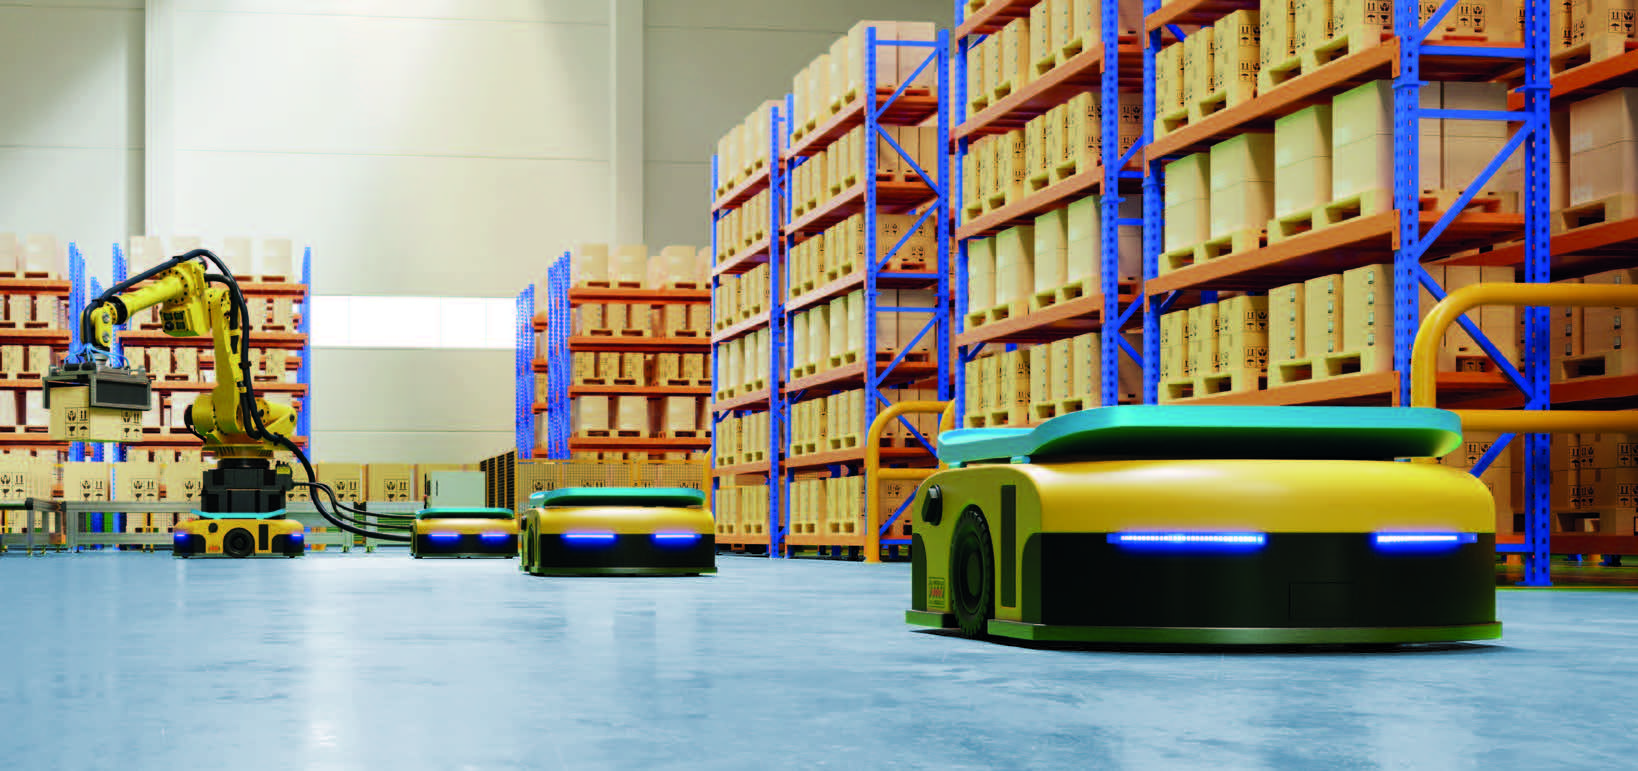
\includegraphics[width=\textwidth]{doc/smart_agv.jpg}
% \caption{Smart AGV in Industry 4.0}
% \end{figure}
% AGVs are essential components in modern industrial automation systems, designed to improve efficiency, flexibility, and safety in material handling and logistics. This section discusses the fundamental theories and principles underlying AGV design, including navigation, control, and system integration.



\end{document}